\documentclass{ctexart}
\usepackage{avanti-color}
\usepackage{avanti-base}
\usepackage{avanti-font}
\usepackage{avanti-math}
\usepackage{avanti-tikz}
\usepackage{avanti-alg}

\begin{document}
\title{算法设计与分析~分治出题}
\author{张腾}
\date{\today}
\maketitle

给定两个$n$位数$x$、$y$,求乘积$z = xy$。记$x = X[0, \ldots, n-1]$、$y = Y[0, \ldots, n-1]$,乘积$z$的长度不超过$2n$,记为$Z[0, \ldots, 2n-1]$。易知有
\begin{align*}
    \sum_{k=0}^{2n-1} Z[k] 10^k = \sum_{i=0}^{n-1} \sum_{j=0}^{n-1} X[i] Y[j] 10^{i+j} = \sum_{k=0}^{2n-2} \underbrace{\sum_{(i,j): i+j=k} X[i] Y[j]}_{c_k} 10^k = \sum_{k=0}^{2n-2} c_k 10^k
\end{align*}
上式左右都是$10^k$的线性组合,但左边的组合系数$Z[k]$是一位正整数,右边的组合系数$c_k$是若干个一位正整数的乘积,因此它们通常并不相等。

第一项$10^0$的系数$c_0 = \sum_{(i,j): i+j=0} X[i] Y[j] = X[0] Y[0]$是个个位数乘积,可能为两位数、也可能为一位数,但不管哪种情况都有$c_0 = \lfloor c_0 / 10 \rfloor \cdot 10 + (c_0 ~ \mod ~ 10)$,其中$h \leftarrow \lfloor c_0 / 10 \rfloor$作为进位会参与到$Z[1]$的计算中,而$c_0 ~ \mod ~ 10$就是$Z[0]$。第二项$10^1$的系数$c_1 = X[0] Y[1] + X[1] Y[0]$是两个个位数乘积的和,可能为三位数、两位数、一位数,此外还要加上进位$h$,最终$h \leftarrow \lfloor (c_1 + h) / 10 \rfloor$作为进位参与$Z[2]$的计算,$(c_1 + h) ~ \mod ~ 10$就是$Z[1]$。如此迭代,继续计算$Z[2], Z[3], \ldots, Z[2n-1]$。

上述正是我们小学所学的乘法,算法1给出了伪代码,该算法通常以填一个$n \times n$二维表的形式实现,图1给出了计算$123 \times 456 = 56088$的例子。

\begin{figure}[h]
    \centering
    \begin{minipage}[t]{0.6\textwidth}
        \centering
        \begin{algorithm}[H]
            \label{alg}
            \caption{$n$位数乘法}
            \begin{algorithmic}[1]
                \Require $X[0, \ldots, n-1]$、$Y[0, \ldots, n-1]$
                \Ensure $Z[0, \ldots, 2n-1]$
                \State 初始化进位$h \leftarrow 0$
                \For {$k = 0 \rightarrow 2n-1$}
                \ForEach {$(i,j): i+j=k$}
                \State $h \leftarrow h + X[i] Y[j]$
                \EndFor
                \State $Z[k] = h ~ (\mod ~ 10)$
                \State $h \leftarrow \lfloor h / 10 \rfloor$ \Comment{下一位的进位}
                \EndFor
            \end{algorithmic}
        \end{algorithm}
    \end{minipage}
    \hfill
    \begin{minipage}[t]{0.36\textwidth}
        \centering
        \vspace{20pt}
        \caption{填表实现}
        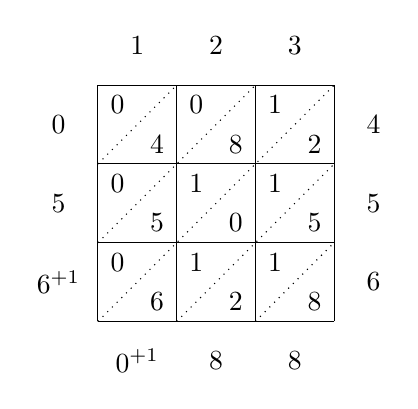
\begin{tikzpicture} []
            \draw (0,0) grid (3,3);
            \draw[dotted] (0,2) -- (1,3);
            \draw[dotted] (0,1) -- (2,3);
            \draw[dotted] (0,0) -- (3,3);
            \draw[dotted] (1,0) -- (3,2);
            \draw[dotted] (2,0) -- (3,1);
            \node () at (0.5,3.5) {$1$};
            \node () at (1.5,3.5) {$2$};
            \node () at (2.5,3.5) {$3$};
            \node () at (3.5,2.5) {$4$};
            \node () at (3.5,1.5) {$5$};
            \node () at (3.5,0.5) {$6$};

            \node () at (2.75,0.25) {$8$};
            \node () at (2.25,0.75) {$1$};
            \node () at (2.75,1.25) {$5$};
            \node () at (2.25,1.75) {$1$};
            \node () at (2.75,2.25) {$2$};
            \node () at (2.25,2.75) {$1$};

            \node () at (1.75,0.25) {$2$};
            \node () at (1.25,0.75) {$1$};
            \node () at (1.75,1.25) {$0$};
            \node () at (1.25,1.75) {$1$};
            \node () at (1.75,2.25) {$8$};
            \node () at (1.25,2.75) {$0$};

            \node () at (0.75,0.25) {$6$};
            \node () at (0.25,0.75) {$0$};
            \node () at (0.75,1.25) {$5$};
            \node () at (0.25,1.75) {$0$};
            \node () at (0.75,2.25) {$4$};
            \node () at (0.25,2.75) {$0$};

            \node () at (0.5,-0.5) {$0^{+1}$};
            \node () at (1.5,-0.5) {$8$};
            \node () at (2.5,-0.5) {$8$};
            \node () at (-0.5,2.5) {$0$};
            \node () at (-0.5,1.5) {$5$};
            \node () at (-0.5,0.5) {$6^{+1}$};
        \end{tikzpicture}
    \end{minipage}
\end{figure}

问题1:算法1第2、3行的二重for循环共遍历$n^2$个$(i,j)$二元组,即二维表中的每一格,因此算法时间复杂度为$\Theta(n^2)$,请设计一种时间复杂度更优的分治算法解决乘法问题。

参考答案:Karatsuba乘法将$x$分成两个$n/2$位数$a$、$b$,将$y$分成两个$n/2$位数$c$、$d$,于是
\begin{align*}
    x = a \cdot 10^{n/2} + b, \quad y = c \cdot 10^{n/2} + d, \quad xy = ac \cdot 10^n + (ad+bc) \cdot 10^{n/2} + bd
\end{align*}
如此会产生$4$个乘法子问题$ac$、$ad$、$bd$、$bc$,根据Strassen乘法的启示:多做加法、少做乘法,利用等式$ad+bc = (a+b)(c+d) - ac - bd$,可将子问题个数减少到$3$个:$ac$、$bd$、$(a+b)(c+d)$,显然加法部分($\Theta(n)$位数相加)复杂度为$\Theta(n)$,因此有递推关系
\begin{align*}
    T(n) = \begin{cases}
               1, & n = 1 \\ 3 \cdot T(n/2) + \Theta(n), & n > 1
           \end{cases}
\end{align*}
利用主定理易知$T(n) = \Theta(n^{\log_2 3})$。

问题2:给定$n$位数$x$,计算$x^2$。最平凡的做法是将平方看作乘法并利用算法1求解,请设计一种时间复杂度更优的分治算法解决平方问题。

参考答案:将$x$二等分成$a$、$b$,即设$x = a \cdot 10^{n/2} + b$,于是$x^2 = a^2 \cdot 10^n + 2ab \cdot 10^{n/2} + b^2$,注意$2ab = (a+b)^2 - a^2 - b^2$,故该分解产生$3$个平方子问题:$a^2$、$b^2$、$(a+b)^2$,显然加法部分复杂度为$\Theta(n)$,因此有递推关系$T(n) = 3 \cdot T(n/2) + \Theta(n)$,与将平方看作乘法并利用Karatsuba乘法求解时间复杂度相同。

\noindent\rule{\textwidth}{0.4pt}

若将$x$三等分,即设$x = a \cdot 10^{2n/3} + b \cdot 10^{n/3} + c$,于是
\begin{align*}
    x^2 & = a^2 \cdot 10^{4n/3} + 2 ab \cdot 10^n + (b^2 + 2ac) \cdot 10^{2n/3} + 2bc \cdot 10^{n/3} + c^2
\end{align*}
注意$2ab = (a+b)^2 - a^2 - b^2$、$2ac = (a+c)^2 - a^2 - c^2$、$2bc = (b+c)^2 - b^2 - c^2$,故该分解产生$6$个平方子问题,有递推关系$T(n) = 6 \cdot T(n/3) + \Theta(n) \Longrightarrow T(n) = \Theta(n^{\log_3 6})$,不及Karatsuba乘法。

\noindent\rule{\textwidth}{0.4pt}

引入多项式$x(t) = a \cdot t^2 + b \cdot t + c$,当$t = 10^{n/3}$时即为$x$,此时
\begin{align*}
    w(t) = x^2(t) & = a^2 \cdot t^4 + 2 ab \cdot t^3 + (b^2 + 2ac) \cdot t^2 + 2bc \cdot t + c^2 \\
                  & \triangleq w_4 \cdot t^4 + w_3 \cdot t^3 + w_2 \cdot t^2 + w_1 \cdot t + w_0
\end{align*}
是$4$次多项式,确定$5$个系数$w_4$、$w_3$、$w_2$、$w_1$、$w_0$再代入$t = 10^{n/3}$即可(相当于每个系数后面依次添加$4n/3$、$n$、$2n/3$、$n/3$、$0$个$0$再相加)。取$t$为$5$个特殊值可得$5$变量线性方程组
\begin{align*}
    \left\{ \begin{array}{lcrcccl}
                t = 0      & : & c^2                          & = & w(0)                & = & w_0                                  \\
                t = 1      & : & (a+b+c)^2                    & = & w(1)                & = & w_4 + w_3 + w_2 + w_1 + w_0          \\
                t = -1     & : & (a-b+c)^2                    & = & w(-1)               & = & w_4 - w_3 + w_2 - w_1 + w_0          \\
                t = 2      & : & (4a+2b+c)^2                  & = & w(2)                & = & 16 w_4 + 8 w_3 + 4 w_2 + 2 w_1 + w_0 \\
                t = \infty & : & \widehat{x}^2 (\infty) = a^2 & = & \widehat{w}(\infty) & = & w_4
            \end{array} \right.
\end{align*}
其中$\widehat{x}(t) = x(t) / t^2$、$\widehat{w}(t) = w(t) / t^4$,求解可得
\begin{align*}
    \left\{ \begin{array}{rcl}
                w_4 & = & a^2                                                            \\
                w_3 & = & (-12 a^2 + (4a+2b+c)^2 - (a-b+c)^2 - 3 (a+b+c)^2 + 3 c^2) / 6  \\
                w_2 & = & (-2 a^2 + (a-b+c)^2 + (a+b+c)^2 - 2 c^2) / 2                   \\
                w_1 & = & (12 a^2 - (4a+2b+c)^2 - 2 (a-b+c)^2 + 6 (a+b+c)^2 - 3 c^2) / 6 \\
                w_0 & = & c^2
            \end{array} \right.
\end{align*}
因此共有$5$个平方子问题:$a^2$、$(4a+2b+c)^2$、$(a-b+c)^2$、$(a+b+c)^2$、$c^2$,时间复杂度$\Theta(n^{\log_3 5})$,优于Karatsuba乘法。

更一般的将$x$作$k$等分,此时$w(t)$是$2k-2$次多项式,共有$2k-1$个系数,线性方程组需包含$2k-1$个方程,由此产生$2k-1$个子问题,时间复杂度$\Theta(n^{\log_k (2k-1)})$。

\end{document}
